\documentclass [aspectratio=169]{beamer}
\beamertemplatenavigationsymbolsempty
\usetheme{Boadilla}
\usepackage{textpos} % package for the positioning
\usepackage[]{graphicx}
\usepackage{graphicx}
\usepackage{float}
\usepackage{hyperref}
\usepackage{caption}
\usepackage{subcaption}
\usepackage{algorithm,algpseudocode}
\usepackage[export]{adjustbox}
\usepackage{tikz}
\usepackage[square,numbers]{natbib}
\usepackage[byname]{smartref}
\usetikzlibrary{positioning}
\usetikzlibrary{arrows, shapes, decorations, automata, backgrounds, fit, petri, calc}

\newcommand*{\logofont}{\fontfamily{phv}\selectfont}

\definecolor{uwopurple}{RGB}{79,38,131} % official blue color for uoft

\title[]{\vspace{40pt} \\
Correlated Shared Frailty Model
Incorporating Ascertainment Correction with Missing Covariates
in Family-Based Studies}
%\subtitle{n}
\author[]{Jiaqi Bi}
%\institute[]{Western University}
\date{Apr. 9, 2024}

% Math notations
\newtheorem{thm}{Theorem}[section]
\newtheorem{lem}[thm]{Lemma}

\newtheorem{defn}[thm]{Definition}
\newtheorem{eg}[thm]{Example}
\newtheorem{ex}[thm]{Exercise}
\newtheorem{conj}[thm]{Conjecture}
\newtheorem{cor}[thm]{Corollary}
\newtheorem{claim}[thm]{Claim}
\newtheorem{rmk}[thm]{Remark}

\newcommand{\ie}{\emph{i.e.} }
\newcommand{\cf}{\emph{cf.} }
\newcommand{\into}{\hookrightarrow}
\newcommand{\dirac}{\slashed{\partial}}
\newcommand{\R}{\mathbb{R}}
\newcommand{\C}{\mathbb{C}}
\newcommand{\Z}{\mathbb{Z}}
\newcommand{\N}{\mathbb{N}}
\newcommand{\Q}{\mathbb{Q}}
\newcommand{\LieT}{\mathfrak{t}}
\newcommand{\T}{\mathbb{T}}
\newcommand{\A}{\mathds{A}}
\newcommand{\E}{\mathbb{E}}
\newcommand{\Prob}{\mathbb{P}}
\newcommand{\Var}{\text{Var}}
\newcommand\equalhat{%
\let\savearraystretch\arraystretch
\renewcommand\arraystretch{0.3}
\begin{array}{c}
\stretchto{
    \scalerel*[\widthof{=}]{\wedge}
    {\rule{1ex}{3ex}}%
}{0.5ex}\\ 
=%
\end{array}
\let\arraystretch\savearraystretch
}

% set color
\setbeamercolor{title in head/foot}{bg=white}
\setbeamercolor{author in head/foot}{bg=white}
\setbeamercolor{date in head/foot}{fg=uwopurple}
\setbeamercolor{date in head/foot}{bg=white}
\setbeamercolor{title}{fg=uwopurple}
\setbeamerfont{title}{series=\bfseries}
\setbeamercolor{frametitle}{fg=uwopurple}
\setbeamerfont{frametitle}{series=\bfseries}
\setbeamercolor{block title}{bg=uwopurple!30,fg=black}
\setbeamercolor{item}{fg=uwopurple}
\setbeamercolor{caption name}{fg=uwopurple!70!}





% set logo at non-title pages
\logo{
\includegraphics[height=0.9cm]{schulich uwo.png}\vspace*{-.055\paperheight}\hspace*{.85\paperwidth}}

\begin{document}

{
\setbeamertemplate{logo}{}
\begin{frame}
    \titlepage
    \begin{textblock*}{4cm}(0.5cm,-7.3cm)
        
\includegraphics[width=4cm]{schulich uwo.png}
    \end{textblock*}
    \begin{textblock*}{8cm}(5.0cm,-7.0cm)
        \huge \color{uwopurple}{$\Bigr\rvert$ \hspace{0.15cm} \textbf{EpiBio Research Day}}
    \end{textblock*}
\end{frame}
}

\begin{frame}{Background}
    \begin{block}{Breast Cancer}
        \begin{itemize}
            \item There were estimated 25,200 new cases of breast cancer in Canada in 2015, and approximately 5,100 deaths, making it the second leading cause of cancer-related death among women~\cite{BCCanadaStatistics2023}.
            \item Hereditary breast-ovarian cancer (HBOC) is an autosomal dominant disease characterized by germline pathogenic mutations in the BRCA1/2 genes~\cite{pritchard2019new}.
            \item Some genetic studies based on the family have been conducted to investigate the hereditary breast cancer and ovarian cancer due to the mutation genes of BRCA1/2~\cite{choi2021association}.
            \item Time-To-Cancer as an outcome, mutation gene status \& PRS are predictors - Problems: There are missing data!
        \end{itemize}
    \end{block}
\end{frame}

\begin{frame}{Pedigree Tree}
    \begin{figure}[!htb]
        \centering
        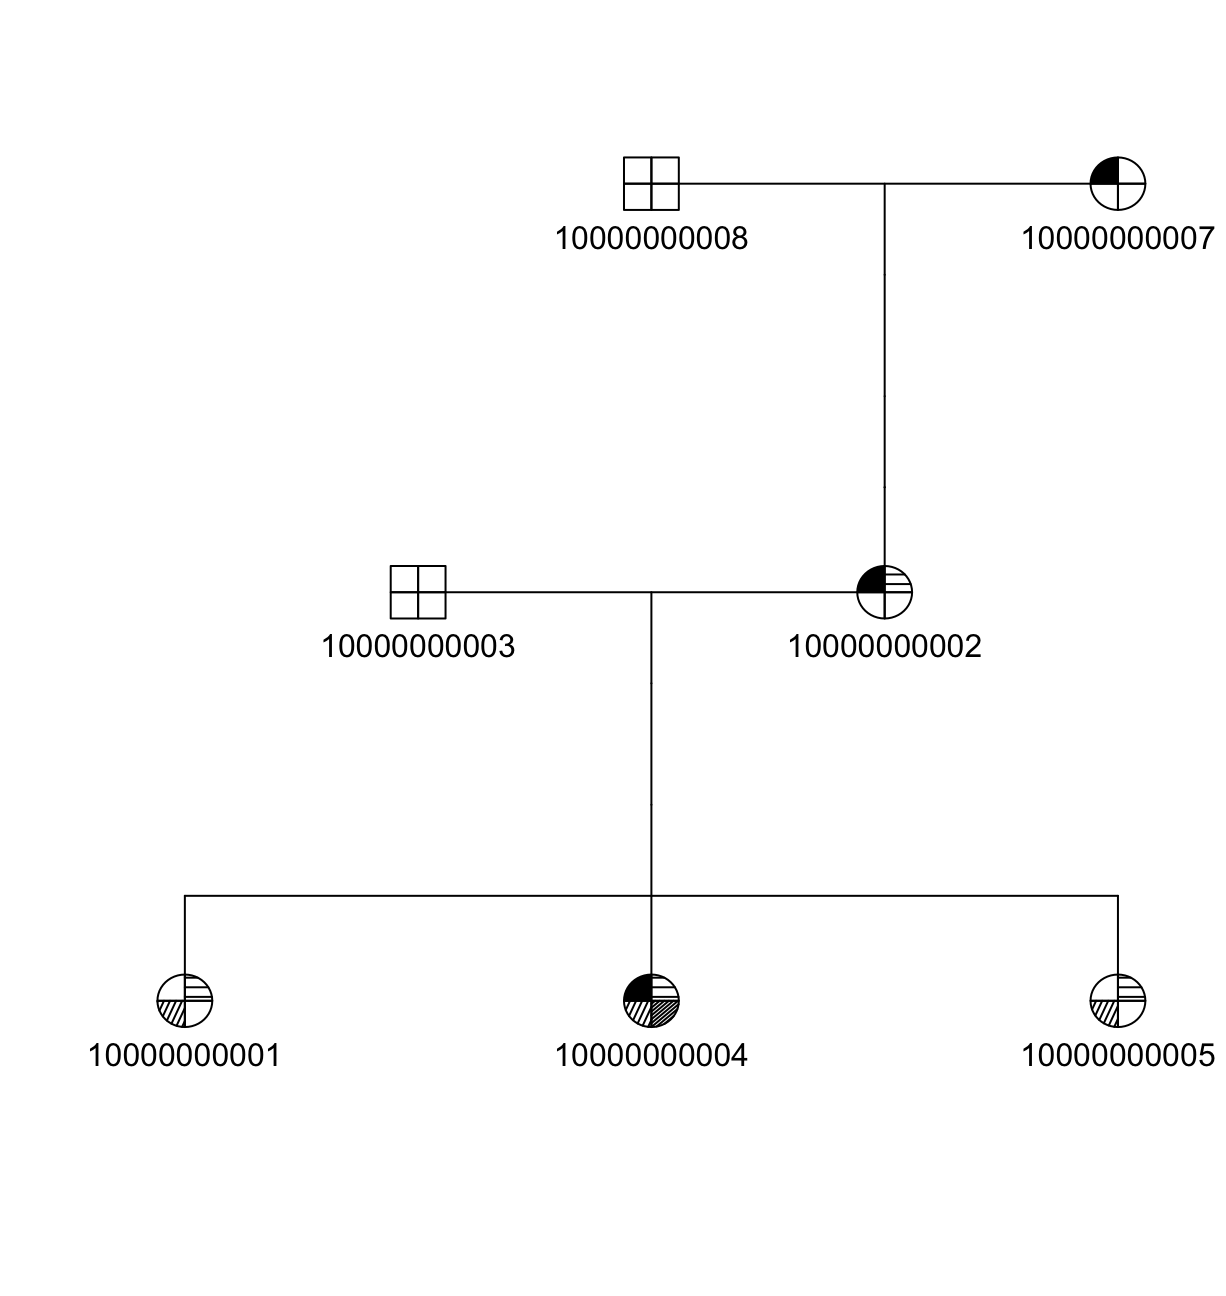
\includegraphics[width=0.5\linewidth]{figures/pedigreetree.png}
        \caption{Pedigree Tree for One Family}
    \end{figure}
\end{frame}

\begin{frame}{Background}
    \begin{block}{Family-Clustered Frailty Model}
        \begin{itemize}
            \item Many different frailty models have been proposed for the analysis of BRCA1/2 families by~\citet{choi2021competing, chen2009frailty}
            \item When the missing data occurs in the frailty model due to other mechanisms than the Missing Completely at Random (MCAR), one may use the Monte Carlo Maximization-Expectation (MCEM)~\cite{herring2002frailty,herring2002maximum,ibrahim2009missing,ripatti2002maximum} or Multiple Imputation (MI)~\cite{rubin2018multiple} methods to make the inference
        \end{itemize}
    \end{block}
    \begin{block}{Missing Data}
        \begin{itemize}
            \item The issue of the missing data was firstly brought by~\citet{rubin1976inference} in 1976.
            \item Three missing mechanisms: MCAR, Missing At Random (MAR), Missing Not At Random (MNAR)
        \end{itemize}
    \end{block}
\end{frame}

\begin{frame}{Missing Mechanisms}
    Denote $Y$ as the complete data matrix, and $M$ as the missing data indicator matrix. 
    Define $y_{ij}$ and $m_{ij}$ as $i$-th row (observation) and $j$-th column (variable) for the matrix $Y$ and $M$. 
    The conditional distribution of the missingness for MCAR is said to be 
    \begin{equation} 
        f(m_{j}|y_{ij}, \phi)=f(m_{ij}|\phi)
    \end{equation}
    The MAR is defined as 
    \begin{equation} 
        f(m_{ij}|y_{ij},\phi)=f(m_{ij}|y_{i,obs}, \phi)
    \end{equation}
    The MNAR is defined as 
    \begin{equation} 
        f(m_{ij}|y_{ij},\phi)=f(m_{ij}|y_{i,mis}, y_{i,obs}, \phi)
    \end{equation}
\end{frame}

\begin{frame}{Parametric Survival Analysis}
    Without loss of generality, everything on the current research will be Weibull baseline hazard. 
    \begin{block}{Weibull Parametric Survival Analysis}
        The hazard function is defined as 
        \begin{equation} 
            h_{ij}(t_{ij}|\mathbf{x}_{ij}, z_j)=h_0(t_{ij})\exp(\boldsymbol{\beta}\mathbf{x}_i)z_j
        \end{equation}
        In our case, for the simplicity, 
        \begin{equation} 
            h_{ij}(t_{ij}|z_j)=h_0(t_{ij})\exp(\beta_1x_{1,ij}+\beta_2 x_{2,ij})z_j
        \end{equation}
        In Weibull baseline hazard, $\lambda$ is the shape parameter, $\alpha$ is the scale parameter
        \begin{equation} 
            h_0(t_{ij})=\alpha\lambda t_{ij}^{\lambda-1}
        \end{equation}
    \end{block}
\end{frame}

\begin{frame}{Complete Likelihood}
    Models are meant to be evaluated on the optimized parameters!
    \begin{block}{Assuming missing data \& frailties are observed}
        \begin{align} 
            L(\boldsymbol{\theta})=\prod_{j=1}^J\prod_{i=1}^{n_j} h(t_{ij}|\mathbf{x}_{ij}, z_j)^{\delta_{ij}}\exp (-H(t_{ij}|\mathbf{x}_{ij},z_j))
        \end{align}
    \end{block}
    \begin{block}{Ascertainment Correction}
        In genetic epidemiology studies, families with multiple affected individuals are more likely to be studied than those with only one or no affected individuals.
        Consider $A$ as the event of being ascertained, we then have $P(D, A|\theta)=P(A|D,\theta)P(D|\theta)$. Thus, we know $A$ is included in $D$, from Baye's rule
        \begin{equation} 
            P(D|\theta)= \frac{P(D,A|\theta)}{P(A|D, \theta)}\propto\frac{L(\theta|D)}{P(A|D,\theta)}
        \end{equation}
    \end{block}
\end{frame}

\begin{frame}{Complete Likelihood}
    \begin{block}{Assuming missing data \& frailties are observed}
        Denote $A(\boldsymbol{\theta})$ be the ascertainment, and $p_j$ be the proband in family $j$, we have 
        \begin{equation} 
            A(\boldsymbol{\theta})=1-S_{p_j}(a_{p_j}|\mathbf{x}_{p_j})
        \end{equation} 
        Then the complete likelihood becomes
        \begin{align} 
            L_C(\boldsymbol{\theta})=\frac{L(\boldsymbol{\theta})}{A(\boldsymbol{\theta})}
        \end{align}
    \end{block}
\end{frame}

\begin{frame}{Complete Log-Likelihood} 
    \begin{block}{Simply take the log} 
        \begin{align} 
            \ell_C(\boldsymbol{\theta})&=\sum_{j=1}^J\sum_{i=1}^{n_j}\delta_{ij}\log h(t_{ij}|\mathbf{x}_{ij}, z_j) - H(t_{ij}|\mathbf{x}_{ij}, z_j)\\
            &-\sum_{j=1}^J \log (1-S_{p_j}(a_{p_j}|\mathbf{x}_{p_j}, z_j)) \\
            &= \sum_{j=1}^J\sum_{i=1}^{n_j}\delta_{ij}\log h(t_{ij}|\mathbf{x}_{ij})z_j - H(t_{ij}|\mathbf{x}_{ij})z_j \\
            &- \sum_{j=1}^{n_j} \log(1- \exp(z_j H_{p_j}(a_{p_j}|\mathbf{x}_{p_j})))
        \end{align}
    \end{block}
\end{frame}

\begin{frame} 
    \begin{block}{Recap on $h(\cdot)$ and $H(\cdot)$} 
        Denote $\xi_{ij}=\exp(\boldsymbol{\beta}^{\top}\mathbf{x}_{ij})$. Note that we can derive 
        \begin{equation} 
            h_{ij}(t_{ij}|\mathbf{x}_{ij}, z_j)=\alpha\lambda t_{ij}^{\lambda-1}\xi_{ij}z_j=h(t_{ij}|\mathbf{x}_{ij})z_j
        \end{equation}
        With one function in the survival analysis, you can derive the rest! So, 
        \begin{align} 
            H(t_{ij}|\mathbf{x}_{ij}, z_j)&=\int_0^{t}h_{ij}(u|\mathbf{x}_{ij}, z_j)du\\
            &=\alpha\xi_{ij}z_j\lambda\int_0^t u^{\lambda-1}du\\
            &=\alpha\xi_{ij}z_j\lambda\cdot \frac{1}{\lambda} t_{ij}^{\lambda}=\alpha\xi_{ij}z_j t_{ij}^{\lambda}=H(t_{ij}|\mathbf{x}_{ij})z_j
        \end{align}
    \end{block}
\end{frame}

\begin{frame}{Frailty Term and Missing Data} 
    \begin{block}{MCAR} 
        If, by any case, one can verify their missing data are MCAR. 
        A complete case analysis (CCA) is enough by MCAR definition. 
        Unfortunately, our data was not this case. 
    \end{block}
\end{frame}

\begin{frame}{Frailty Distributions}
    If we assume $z_j\sim\text{Gamma}(\upsilon, \upsilon)$, as shape and rate parameters. then the likelihood will look like these
    \begin{figure}[!htb]
        \centering
        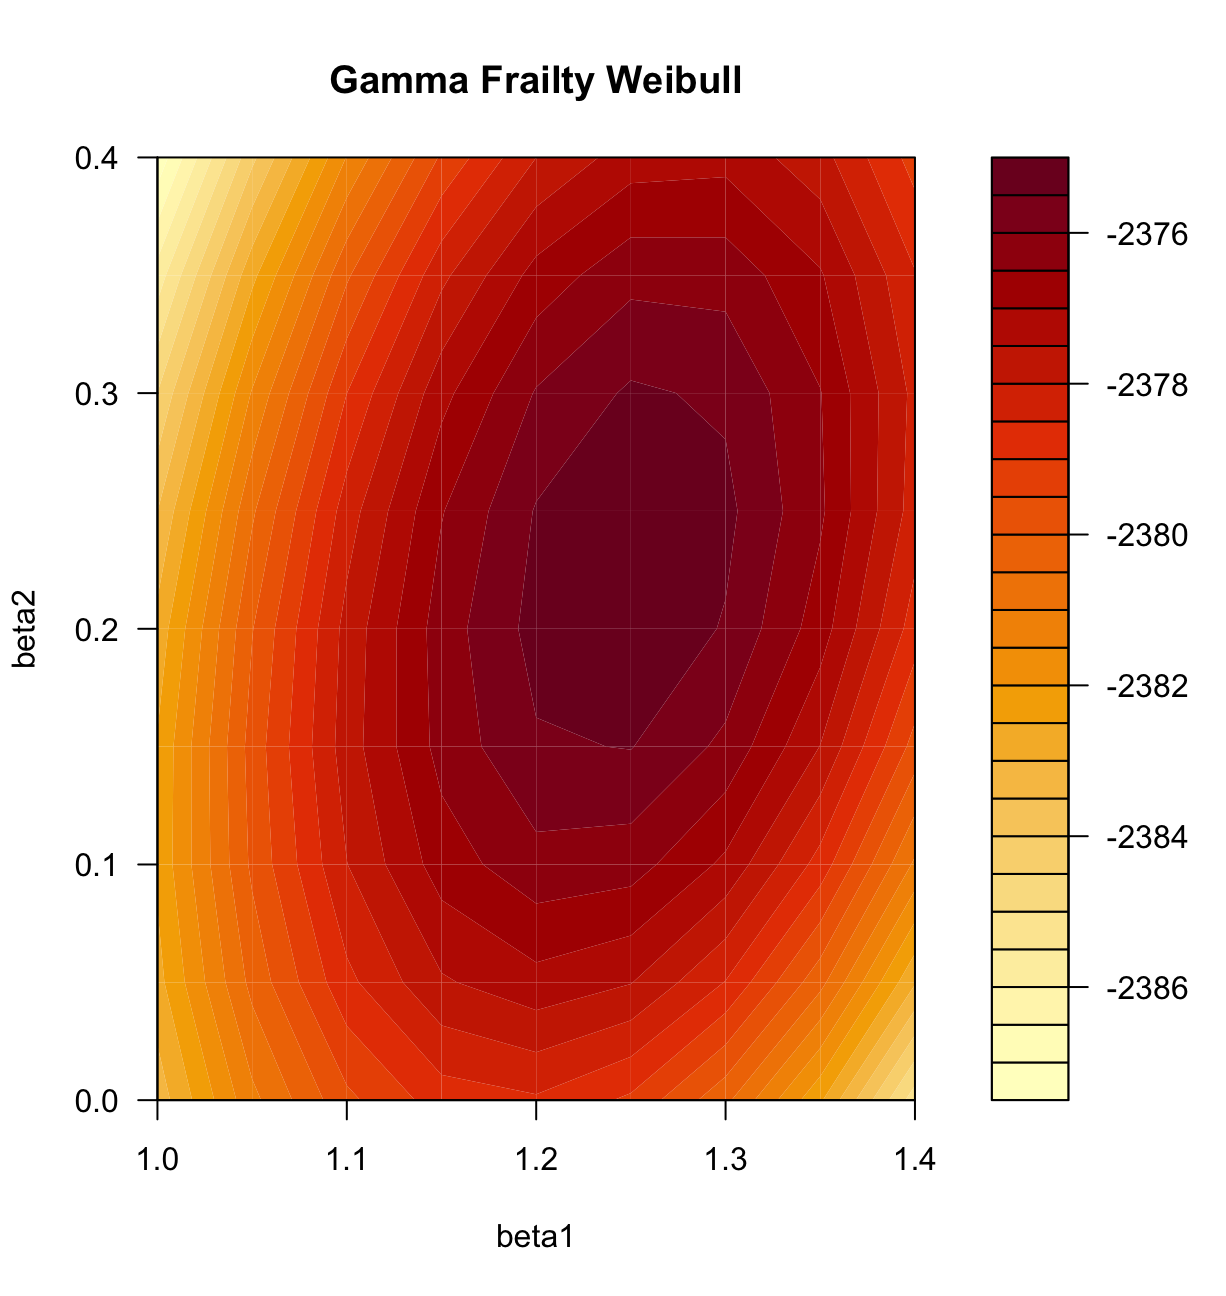
\includegraphics[width=0.5\linewidth]{figures/gamma contour.png}
        \caption{Contour Plot for Gamma Frailty}
    \end{figure}
\end{frame}

\begin{frame}{Frailty Distributions}
    If we assume $z_j\sim\text{Gamma}(\upsilon, \upsilon)$, as shape and rate parameters. then the likelihood will look like these
    \begin{figure}[!htb]
        \centering
        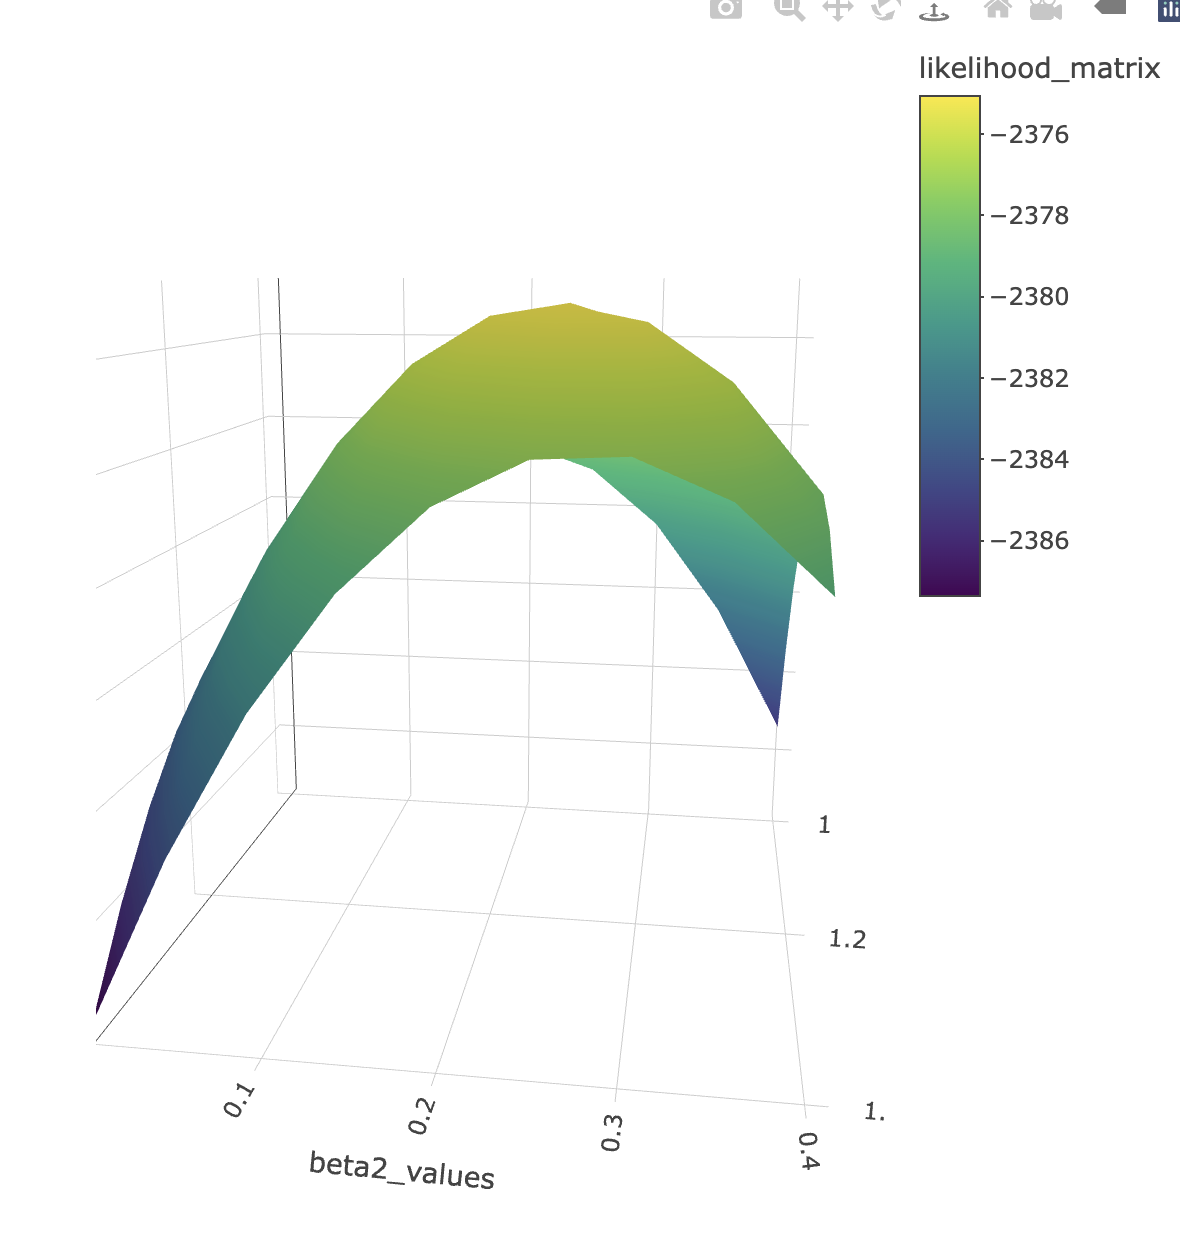
\includegraphics[width=0.5\linewidth]{figures/GAMMA 3D 1.png}
        \caption{3D Contour Plot for Gamma Frailty 1}
    \end{figure}
\end{frame}

\begin{frame}{Frailty Distributions}
    If we assume $z_j\sim\text{Gamma}(\upsilon, \upsilon)$, as shape and rate parameters. then the likelihood will look like these
    \begin{figure}[!htb]
        \centering
        \includegraphics[width=0.5\linewidth]{figures/GAMMA 3D 2.png}
        \caption{3D Contour Plot for Gamma Frailty 2}
    \end{figure}
\end{frame}


\begin{frame}{Frailty Distributions}
    If we assume $z_j\sim\text{logN}(0,\upsilon^2)$, then the likelihood will look like these
    \begin{figure}[!htb]
        \centering
        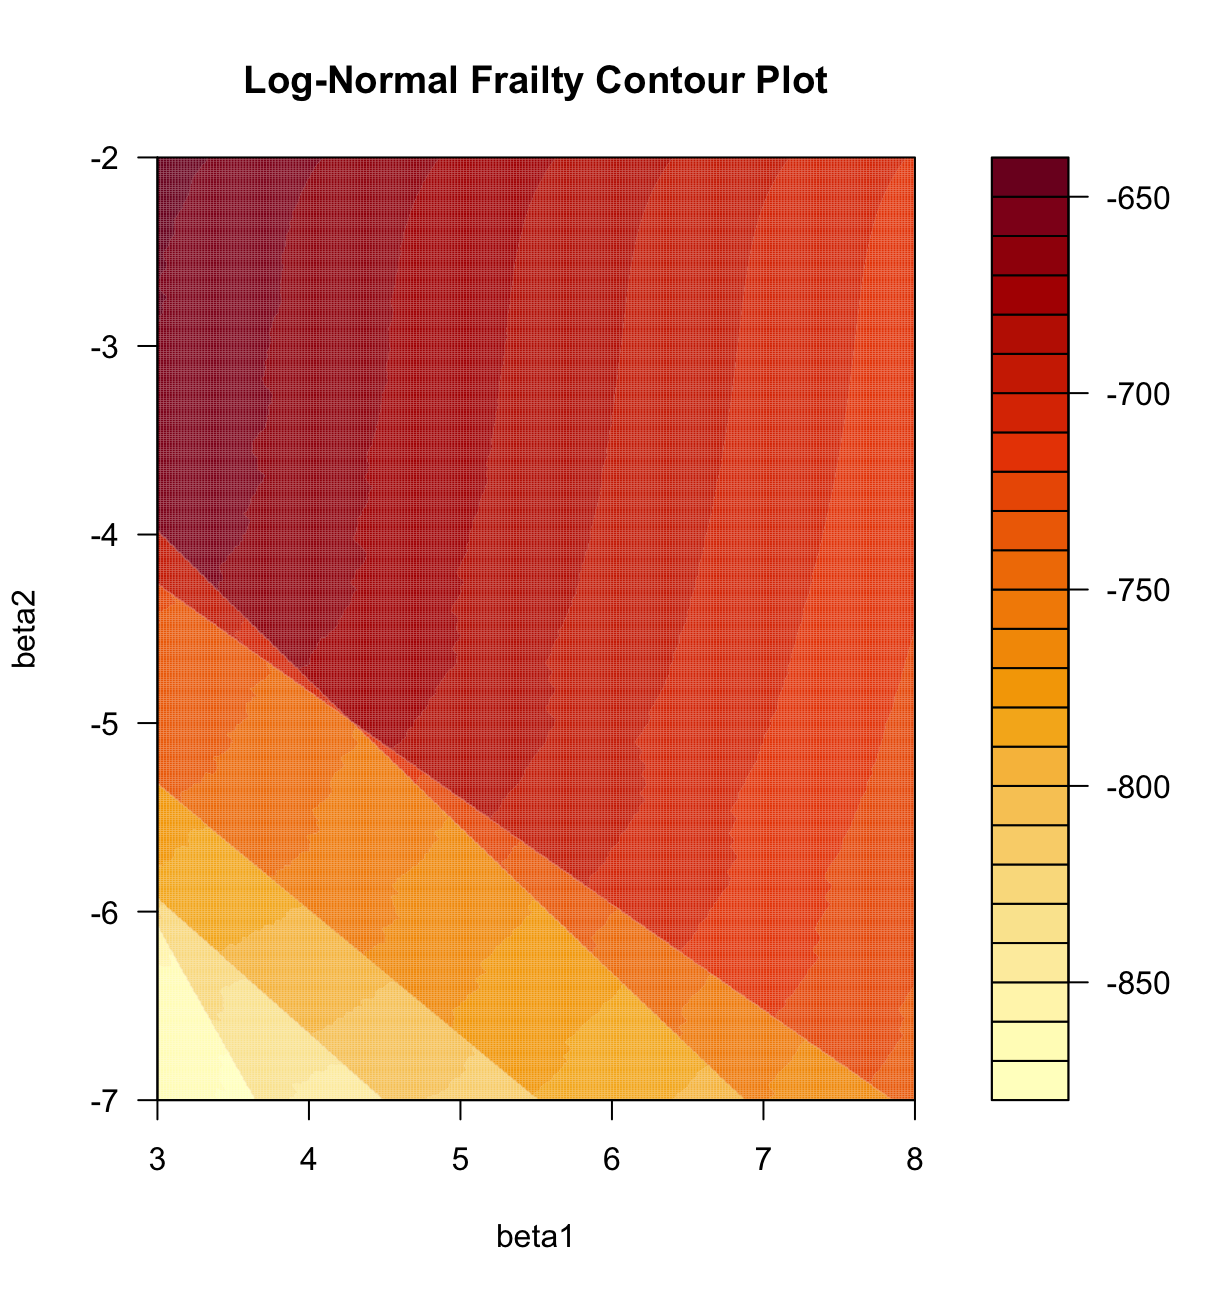
\includegraphics[width=0.5\linewidth]{figures/lognormal frailty contour.png}
        \caption{Contour Plot for Log-Normal Frailty}
    \end{figure}
\end{frame}

\begin{frame}{Frailty Distributions}
    \begin{figure}[!htb]
        \centering
        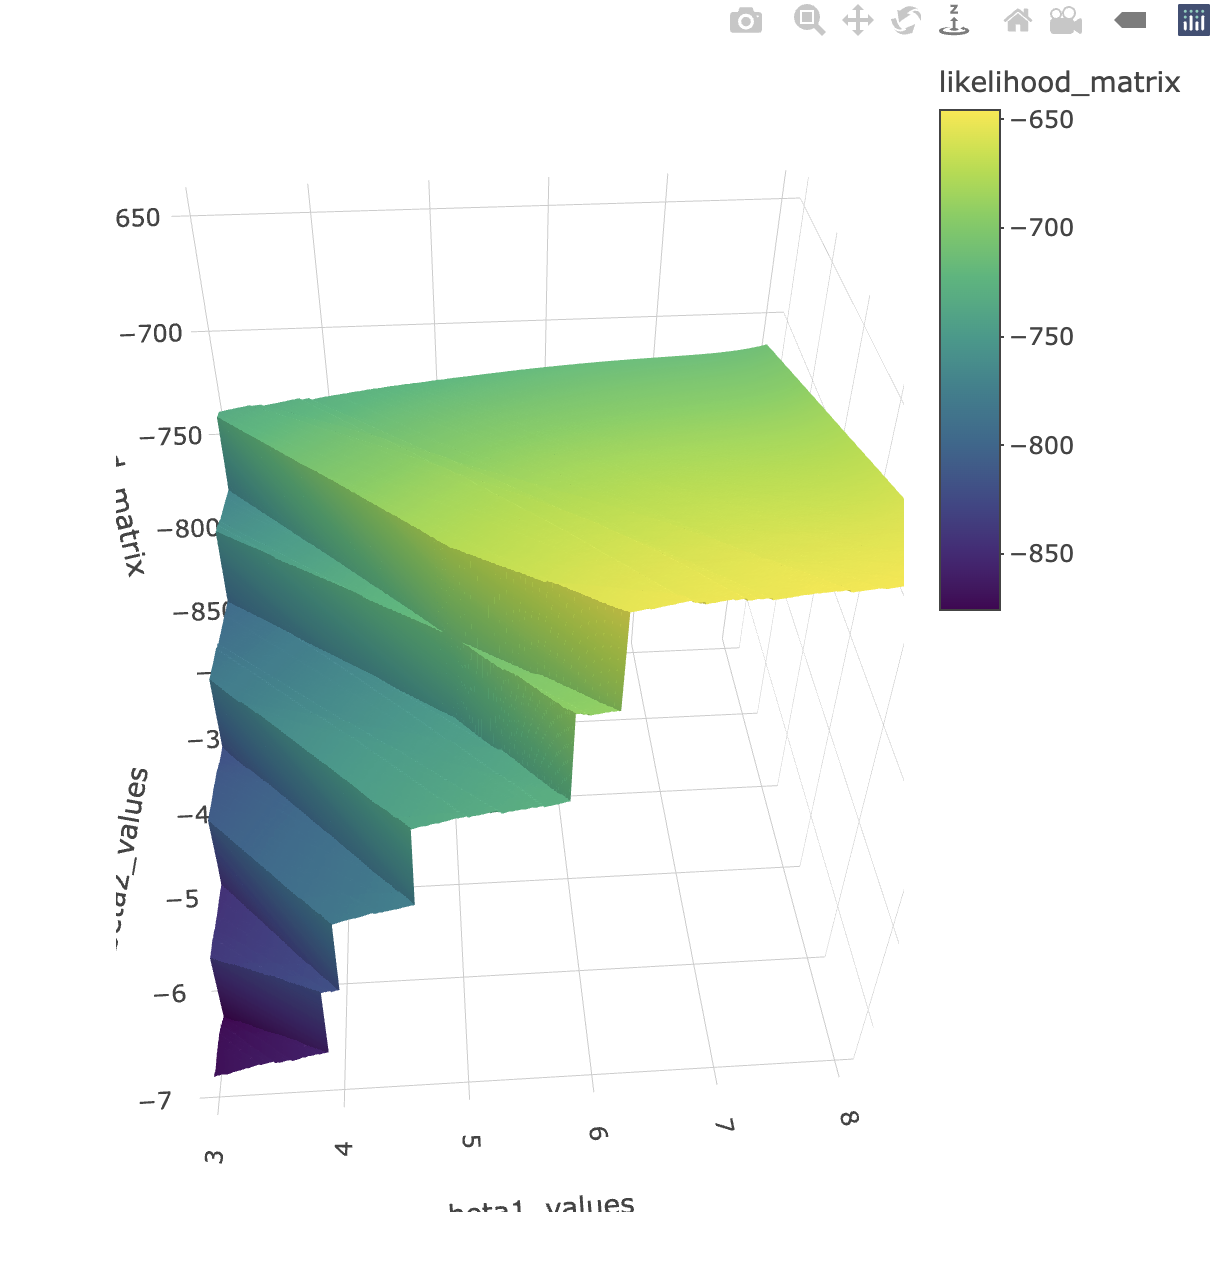
\includegraphics[width=0.5\linewidth]{figures/lognormal frailty 3D 1.jpeg}
        \caption{3D Contour Plot for Log-Normal Frailty 1}
    \end{figure}
\end{frame}

\begin{frame}{Frailty Distributions}
    \begin{figure}[!htb]
        \centering
        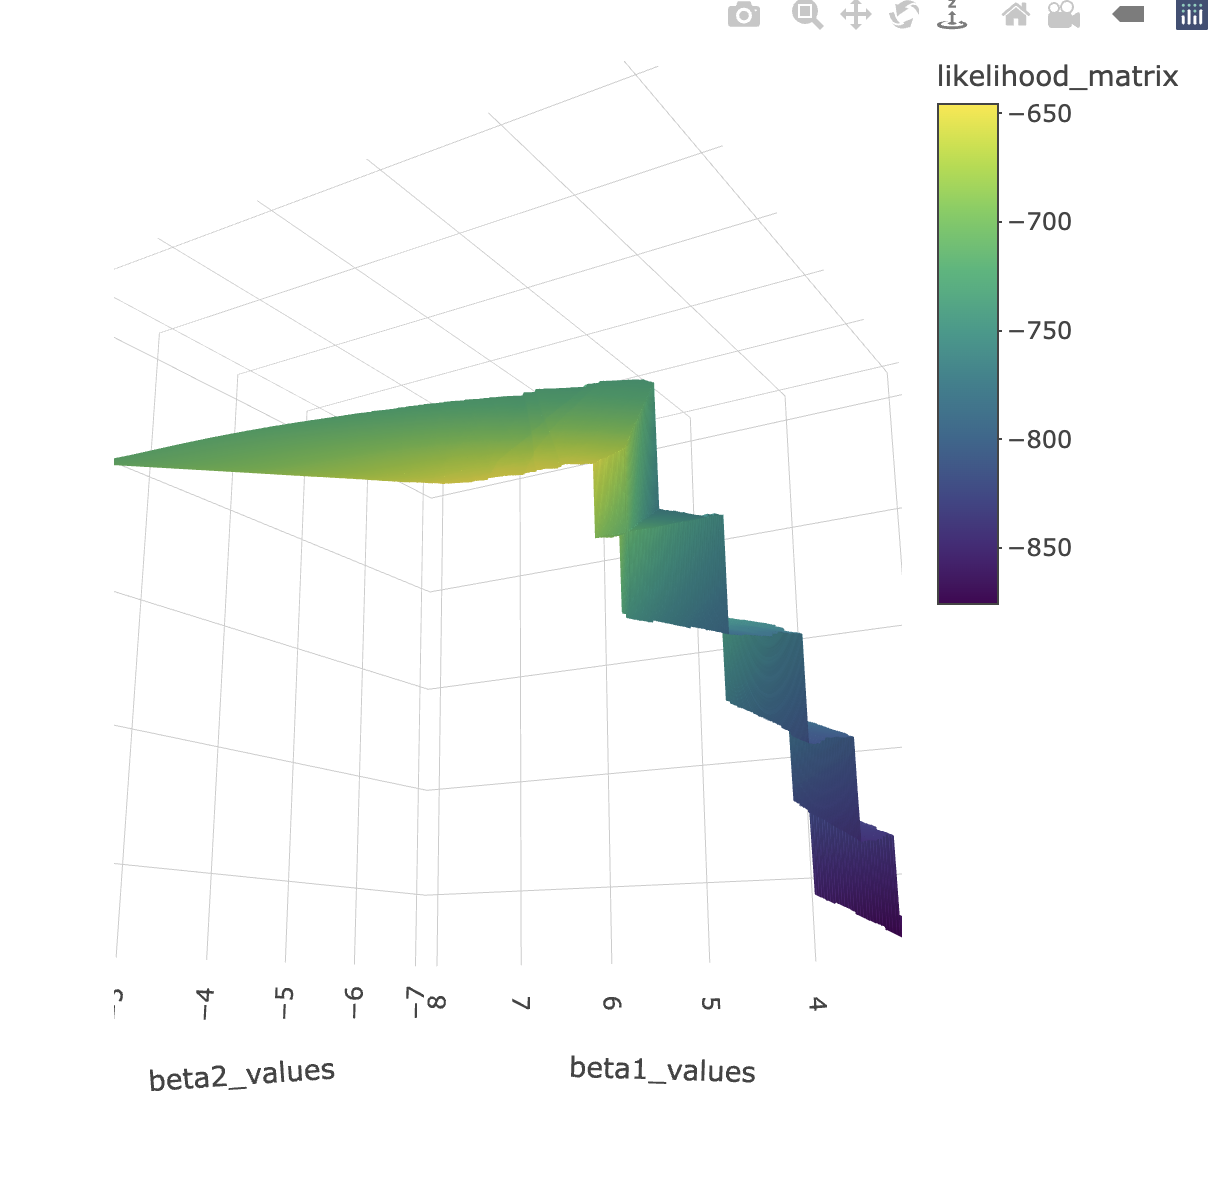
\includegraphics[width=0.5\linewidth]{figures/lognormal frailty 3D 2.jpeg}
        \caption{3D Contour Plot for Log-Normal Frailty 2}
    \end{figure}
\end{frame}

\begin{frame}{Frailty Term and Missing Data}  
    \begin{block}{MAR}
        However, the MCAR is a very strong assumption, and usually not verified. 
        By definition, we need to take the expectation with respect to the frailty term $z_j$ and the missing data $\mathbf{x}_{ij,mis}$. 
        Assume the frailty distribution is chosen to be $f(z_j|\upsilon)$, and one might take the missing PRS $x_{ij,1,mis}\sim N(\psi_0+\psi_1x_{ij,2,obs}, \tilde{\psi}^2)$ to sample from. 
        \begin{align} 
            E(\ell_C(\boldsymbol{\theta})|\boldsymbol{\theta}^{(r)})=&\sum_{j=1}^J\sum_{i=1}^{n_j}\int_{\mathbf{x}_{mis}} \int_{z_j}\Big (\delta_{ij}\log h(t_{ij}|\mathbf{x}_{ij}, z_j) - H(t_{ij}|\mathbf{x}_{ij}, z_j)\Big )\\
            &\times f(\mathbf{x}_{ij,mis}|\mathbf{x}_{obs,ij},\psi^{(r)})f(z_j|\upsilon^{(r)})d\mathbf{x}_{ij,mis}dz_j\\
            &-\sum_{j=1}^J \int_{\mathbf{x}_{mis}} \int_{z_j} \log(1- \exp(z_j H_{j_p}(a_{j_p}|\mathbf{x}_{j_p})))\\
            &\times f(\mathbf{x}_{ij,mis}|\mathbf{x}_{obs,ij},\psi^{(r)})f(z_j|\upsilon^{(r)})d\mathbf{x}_{ij,mis}dz_j
        \end{align}
    \end{block}
\end{frame}

\begin{frame}{Gamma Frailty Term and Missing Data} 
    We can integrate $z_j$ in Gamma frailty via Laplace transform, assuming $z_j\sim\text{Gamma}(k,k)$, which will yield a closed-form likelihood
    \begin{equation} 
        \ell(\boldsymbol{\theta})=\sum_{j=1}^J\left [\sum_{i=1}^{n_j}(\delta_{ij}\log h(t_{ij}|\mathbf{x}_{ij})) + \log\Big (\frac{(k+d_j-1)!}{k!k^{d_j-1}}(1+\frac{\sum_{i=1}^{n_j}(H(t_{ij}|\mathbf{x}_{ij}))}{k})^{-k-d_j}\Big )\right ]
    \end{equation}
    The ascertainment term 
    \begin{align} 
    A_j(\boldsymbol{\theta})&=1-S_{p_j}(a_{p_j}|\mathbf{x}_{p_j})\\
    &=1-\int_0^{\infty} S_{p_j}(a_{p_j}|\mathbf{x}_{p_j},z_j)f(z_j)dz_j\\
    &=1-\int_0^{\infty}\exp(-z_j\cdot H_{p_j}(a_{p_j}|\mathbf{x}_{p_j}))f(z_j)dz_j\\
    &=1-(1+\frac{H_{p_j}(a_{p_j}|\mathbf{x}_{p_j})}{k})^{-k}
    \end{align}
\end{frame}

\begin{frame}{Log-Normal Frailty Term and Missing Data} 
    We can integrate $z_j$ in Log-Normal frailty via Gauss-Hermite Quadrature, which will yield a closed-form likelihood
    \begin{definition} 
        In numerical analysis, the method can be applied in the following form:
        \begin{equation}
            \int_{-\infty}^{\infty}\exp(-x^2)f(x)dx\approx \sum_{i=1}^n\omega_i f(x_i)
        \end{equation}
        where $n$ is number of sample points used, and $x_i$ is the roots of Hermite polnomial $H_n (x)$ such that $i=1, ..., n$, and the weights $\omega_i$ is 
        \begin{equation}
            \omega_i=\frac{2^{n-1}n!\sqrt{n}}{n^2[H_{n-1}(x_i)]^2}
        \end{equation}
    \end{definition}
\end{frame}

\begin{frame}{Log-Normal Frailty Term and Missing Data}
    $q$ denotes the $q$-th element of Gauss Hermite Quadrature, i.e., $\omega_{q}$ denotes the $q$-th weight, $y_{q}$ denotes the $q$-th node, and $N_{q}$ denotes the total number of quadratures. Thus, substituting into the log-likelihood:
    \begin{equation}
        \ell_j(\boldsymbol{\theta})=\sum_{i=1}^{n_j}\delta_{ij}\log(h(t_{ij}|\mathbf{x}_{ij}))+\log\Big (\frac{1}{\sqrt{\pi}}\sum_{q=1}^{N_{q}}\left [\omega_{q}\exp(\sqrt{2}\sigma y_{q})^{d_j}\exp\Big (-\sum_{i=1}^{n_j}H(t_{ij}|\mathbf{x}_{ij})\exp(\sqrt{2}\sigma y_{q})\Big )\right ]\Big )
    \end{equation}
    Similarly, the ascertainment correction in the log-normal frailty can be written as 
    \begin{align}
        A_j(\boldsymbol{\theta})&=1-\int_{-\infty}^{\infty} \exp(-z H(a_{j_p}|\mathbf{x}_{j_p}))f(z)dz\\
        &=1-\sum_{q=1}^{N_{q}}\omega_{q} \exp\left (-(\sum_{i=1}^{n_j} H(a_{j_p}|\mathbf{x}_{j_p}))\exp (\sqrt{2}\sigma y_{q_p})\right )
    \end{align}
\end{frame}

\begin{frame}{Frailty Term and Missing Data}
    \begin{equation} 
        \ell_{C_{j}}=\ell_j(\boldsymbol{\theta})-\log A_j(\boldsymbol{\theta})
    \end{equation}
\end{frame}

\begin{frame}{Frailty Term and Missing Data - Monte Carlo Expectation Maximization (MCEM)}
    For efficient sampling on missing data, 
    \begin{align} 
        f(z_j, \mathbf{x}_{mis,ij}|\mathbf{x}_{obs,ij}, \boldsymbol{\theta}^{(r)})&\propto f(t_{ij}, \delta_{ij}|\mathbf{x}_{mis,ij}, \mathbf{x}_{obs,ij}, z_j, a_{j_p}, \boldsymbol{\beta}^{(r)})\\
        &\times f(\mathbf{x}_{mis,ij}|\mathbf{x}_{obs,ij}, \psi^{(r)})f(z_j|\upsilon^{(r)})
    \end{align}
    Clearly, we know $f(t_{ij}, \delta_{ij}|\mathbf{x}_{mis,ij}, \mathbf{x}_{obs,ij}, z_j, \boldsymbol{\beta}^{(r)})$ is the likelihood of one single observation $j$ in family $j$, also we know the distribution of $f(\mathbf{x}_{ij}|\psi)$, as well as the frailty distribution $f(z_j|\upsilon)$. 
    Therefore, in our case, we can write 
    \begin{align} 
        f(z_j, \mathbf{x}_{mis,ij}|\mathbf{x}_{obs,ij}, \boldsymbol{\theta}^{(r)})&\propto f(z_j|\upsilon^{(r)})\Big [ \prod_{i=1}^{n_j} f(\mathbf{x}_{mis,ij}|\mathbf{x}_{obs,ij}, \psi^{(r)})\\ 
        &\times h^{(r)}(t_{ij}|\mathbf{x}_{ij}, z_j)^{\delta_{ij}}\exp (-H^{(r)}(t_{ij}|\mathbf{x}_{ij}, z_j))\Big ]
    \end{align}
\end{frame}

\begin{frame}{Frailty Term and Missing Data - MCEM}
    In general, without the specification of the frailty distribution, the E-step in MCEM can be written as 
    \begin{align} 
        Q(\boldsymbol{\theta}|\boldsymbol{\theta}^{(r)})
        &=\sum_{j=1}^J \frac{1}{M_j}\sum_{m=1}^{M_j}\sum_{i=1}^{n_j} \Big ( \delta_{ij}\log h(t_{ij}|\mathbf{x}_{ij}^{(m)}, z_j^{(m)}) - H(t_{ij}|\mathbf{x}_{ij}^{(m)}, z_j^{(m)})\Big )\\
        &+\sum_{j=1}^J\frac{1}{M_j}\sum_{m=1}^{M_j}\log(1- \exp(z_j H_{j_p}(a_{j_p}|\mathbf{x}_{j_p})))\\
        &+\sum_{j=1}^J\frac{1}{M_j}\sum_{m=1}^{M_j}\sum_{i=1}^{n_j}\log f(\mathbf{x}_{mis,ij}^{(m)}|\mathbf{x}_{obs,ij}, \psi)+\sum_{j=1}^J\frac{1}{M_j}\sum_{m=1}^{M_j}\sum_{i=1}^{n_j}\log f(z_j^{(m)}|\upsilon)
    \end{align} 
    Note that we take $M_j$ samples of the missing data and calculate the mean. 
\end{frame}

\begin{frame}{Kinship Matrix}
    Remember, we made an assumption of the distribution of the missing PRS:
    \begin{equation} 
        x_{ij,1,mis}\sim N(\psi_0+\psi_1x_{ij,2,obs}, \tilde{\psi}^2) 
    \end{equation} 
    Is this an adequate assumption? 
\end{frame}

\begin{frame}{Kinship Matrix}
    No! This is a family-wise genetic study! So within-family correlations need to be accounted for! 
    \begin{equation}
        \mathbf{x}_{mis,j,1}\sim MVN(\boldsymbol{\mu}, \tilde{\psi}_g^2K+\tilde{\psi}_e^2)
    \end{equation}
    such that $K$ is the kinship correlation matrix with diagonal of 1, and $\hat{\boldsymbol{\mu}}=\boldsymbol{\psi}_0+\boldsymbol{\psi}_1 \mathbf{x}_{obs,j,2}$. 
    $\tilde{\psi}_g$ accounts for the genetic standard errors, and $\tilde{\psi}_e$ accounts for the residual. 
    The multivariate normal distribution is what we are sampling the missing PRS on family-wise. 
\end{frame}

\begin{frame}{Frailty Term and Missing Data - MCEM} 
    \begin{block}{M-Step}
        In the M-step, I will use Nelder-Mead method, because it is gradient free! 
    \end{block}
    \begin{block}{Convergence Rule}
        The convergence criterion is 
        \begin{equation} 
            (\boldsymbol{\theta}^{(r+20)}-\boldsymbol{\theta}^{(r)})^2 < 10^{-4}
        \end{equation}
    \end{block}
\end{frame}

\begin{frame}{Preliminary Analysis Results} 
    \begin{table}[]
        \caption{Parameter Estimates on BRCA1 Family (MCEM - Assumed MAR)}
        \begin{tabular}{lllll}
        \hline
        Parameters & Gamma (CCA) & Log-Normal (CCA) & Gamma (MCEM) & Log-Normal (MCEM) \\ \hline
        $\alpha$   & -4.10               & -10.91                   & -4.71                & -19.05                    \\
        $\lambda$  & 1.06                & 1.41                     & 0.84                 & 1.12                      \\
        $\beta_1$  & 1.26                & -5.12                    & 2.42                 & 3.97                      \\
        $\beta_2$  & 0.23                & 6.62                     & 0.34                 & 0.42                      \\
        $\upsilon$ & 4.35                & 2.73                     & 3.71                 & 2.89                      \\ \hline
        \end{tabular}
        \end{table}
        The Log-normal distribution can introduce a wider range of heterogeneity due to its ability to model right-skewed distributions effectively. 
        This wider range means that, once the Log-Normal frailty is accounted for, the remaining baseline hazard needs to adjust significantly to fit the data, hence the more negative scale parameter.
        A smaller (more negative) scale parameter indicates a more rapid initial occurrence of events, with the rate of increase over time again depending on the shape parameter.
\end{frame}

\begin{frame}{Next Step} 
    \begin{itemize} 
        \item Due to the computational cost - The MCEM runs 48+ hours, I have not obtained the preliminary result on the case of the MNAR, but I will.
        \item A simulation study based on the correlated family will be conducted. 
        \item Stay tuned for the final thesis! 
    \end{itemize}
\end{frame}

\begin{frame}[t,allowframebreaks]{References}
    \bibliographystyle{unsrtnat}
    \bibliography{ref.bib}
\end{frame}

\begin{frame}{Q\&A}
    Question Time!
\end{frame}

\end{document}